\section{Demonstration}
% \meta{Briefly show screenshots and how the server works and is distributed}
For ease of use, Yarn exposes a help command to show the options available
when launching the server. Figure~\ref{screenshot} shows the output of the
help command.

\begin{figure}[htb]
  \centering
  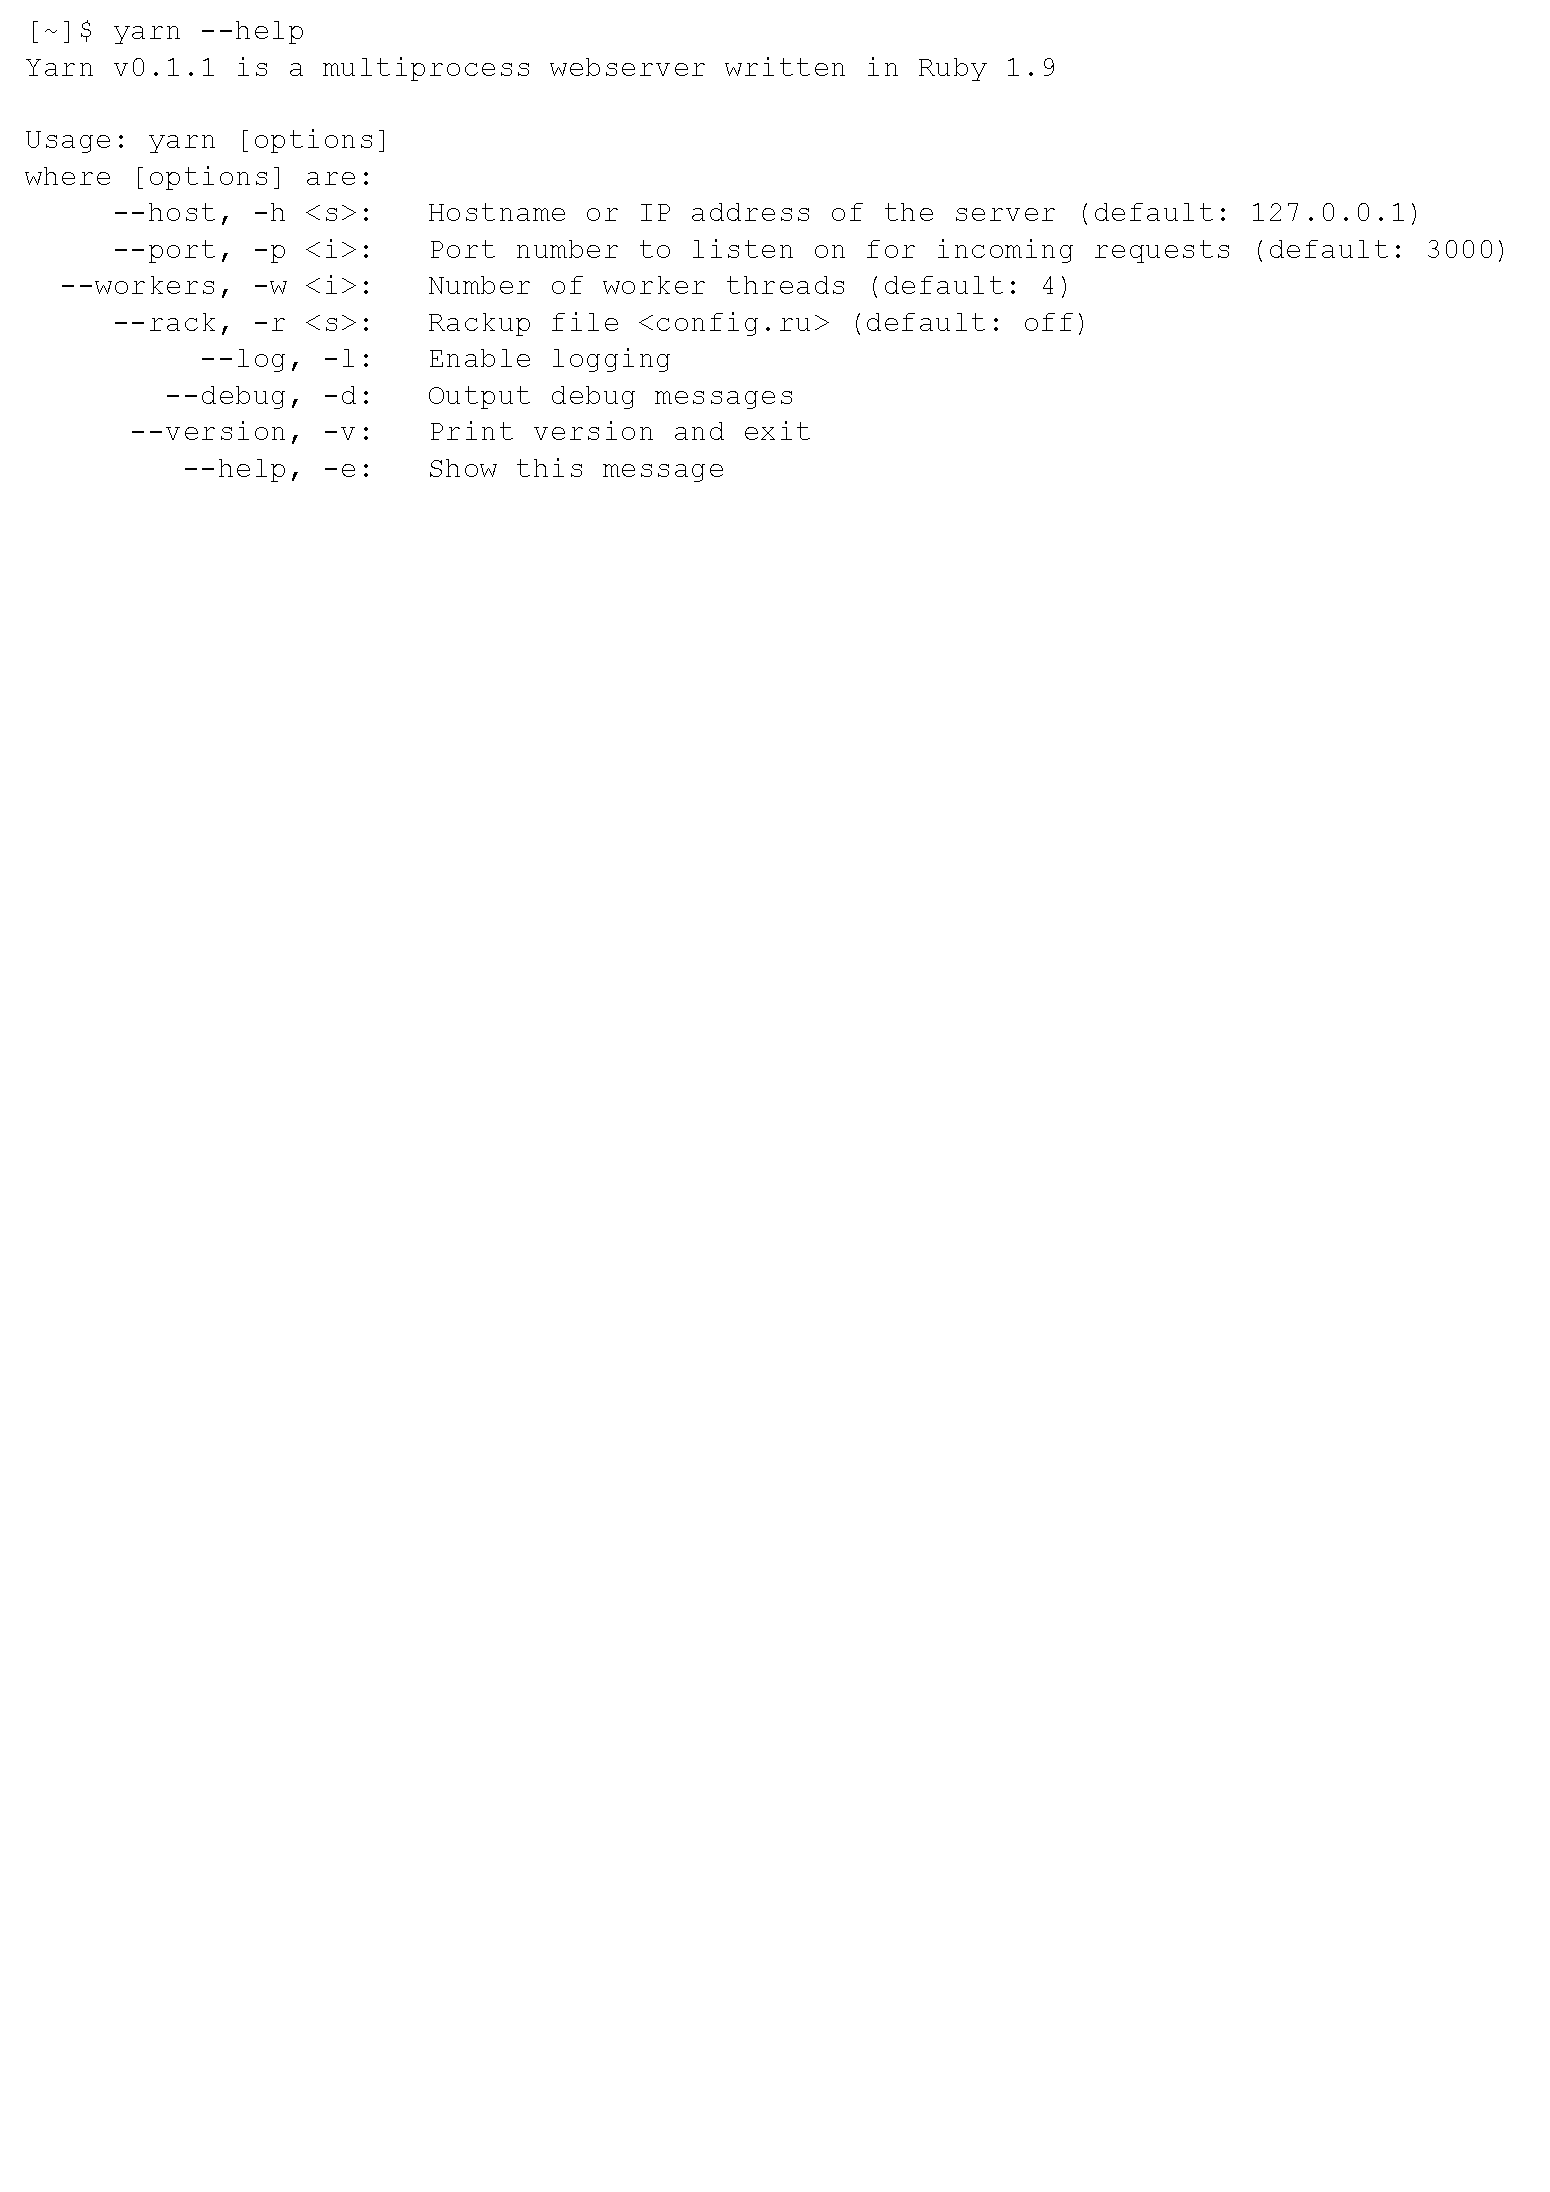
\includegraphics[width=0.85\textwidth]{img/yarnhelp.pdf}
  \caption{Yarn help output.}
  \label{screenshot}
\end{figure}

Figure~\ref{screenshot2} shows the output when Yarn is serving static and Ruby
files with 32 worker processes and logging enabled.

\begin{figure}[htb]
  \centering
  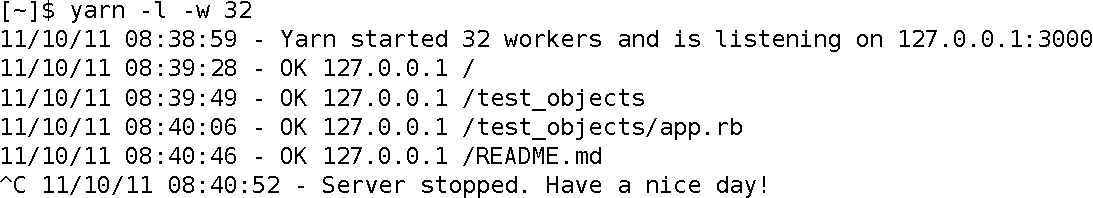
\includegraphics[width=0.8\textwidth]{img/yarnserve.pdf}
  \caption{Yarn static/dynamic output.}
  \label{screenshot2}
\end{figure}

Figure~\ref{screenshot3} shows Yarn serving a sample Ruby on Rails
application.

\begin{figure}[htb]
  \centering
  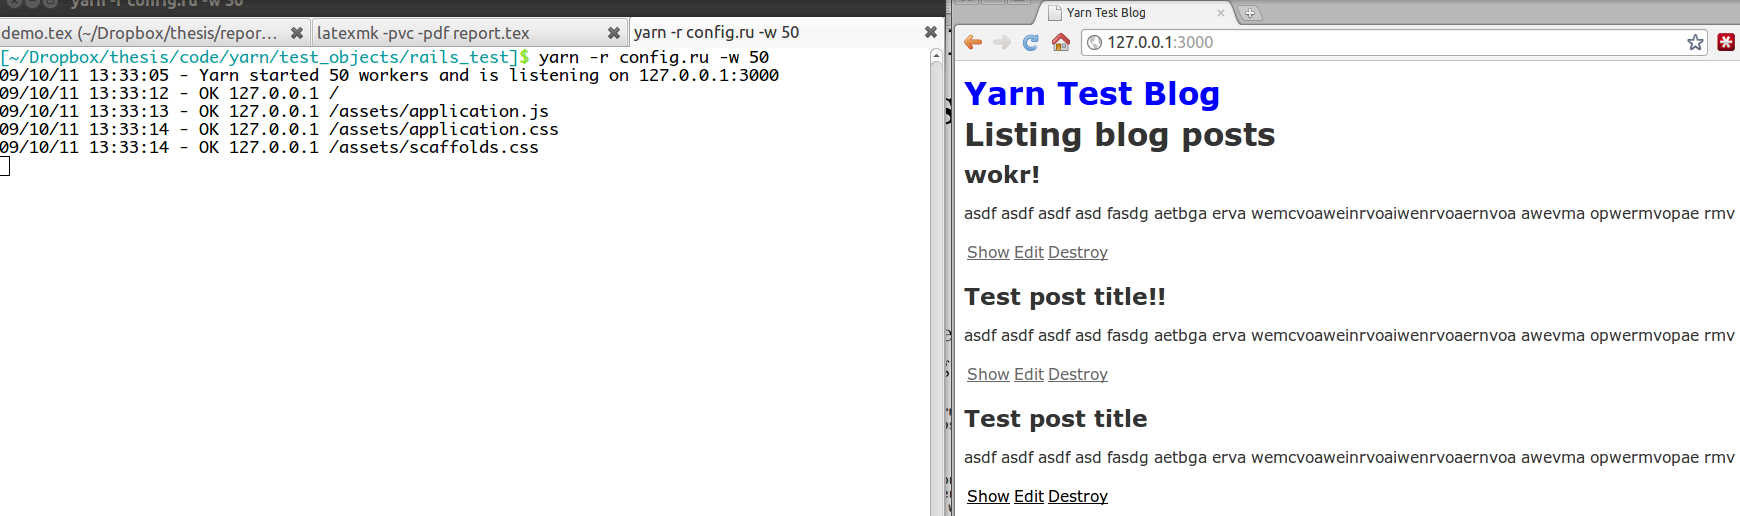
\includegraphics[width=1.0\textwidth]{img/scr3.png}
  \caption{Yarn Rack application output.}
  \label{screenshot3}
\end{figure}

Yarn can easily be installed using RubyGems which is included in Ruby as of
version 1.9. To install Yarn run the following command \texttt{gem install
  yarn}, and now Yarn is available from the command-line. 

